\section{Theorie}
\label{sec:Theorie}


Bei natürlichen Prozessen ist zu beobachten, dass die höhere Temperatur sich immer auf die niedrigere Temperatur zubewegt.
Der erste Hauptsatz der Thermodynamik besagt, dass Temperatur eine Energieform ist, deren Fließrichtung durch Hinzunahme von Arbeit umkehrbar ist. 
Eine solche Arbiet $A$ wird bei der Wärmepumpe in Form von mechanischer Arbeit durch den Kompressor verrichtet.

\subsection{Aufbau}

\begin{figure} 
    \centering
    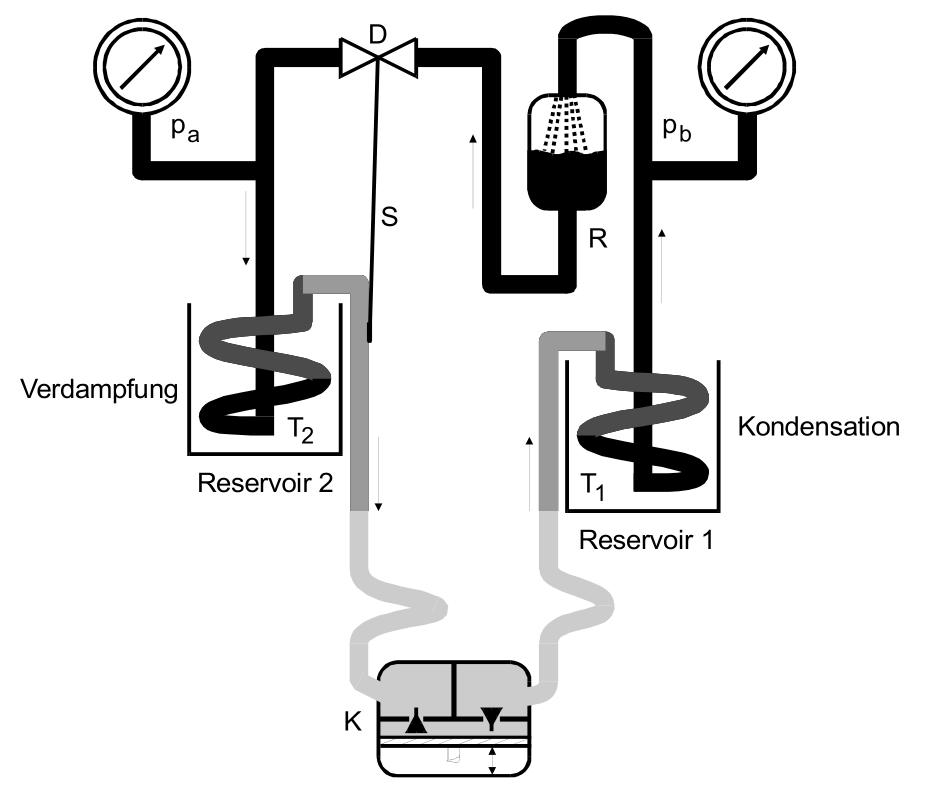
\includegraphics[width=8cm] {pictures/Aufbau.png} \cite{v206} 
    \caption{Prinzipieller Aufbau einer Wärmepumpe}
    \label{fig:aufbau_wärmepumpe}
\end{figure} 


In \ref{fig:aufbau_wärmepumpe} ist der Kompressor $K$, die beiden Reservoirs 1 und 2, die Drossel $D$, der Reiniger $R$ und die beiden 
Druckmessgeräte $P_{a}$ und $P_{b}$ zu erkennen, welche durch Leitungen verbunden sind. Innerhalb dieser Leitungen fließt das 
Transportmedium. Dabei handelt es sich um das Gas Dichlordifluormethan ($\ce{Cl2F2C}$). Dieses wird sich je nach Lage verflüssigen oder verdampfen. 
Beim verdampfen nimmt das Gas Verdampfungswärme auf und beim verflüssigen gibt es diese ab. \\

Im Aufbau der Skizze ist das wärmeabgebende (flüssige) Reservoir das Reservoir 2 mit $T_{2}$ und $p_{a}$. Demnach ist Reservoir 1 das wärmeaufnehmende
(gasförmige) Reservoir mit der Temperatur $T_{1}$ und $p_{b}$. \\

Der Kompressor $K$ erzeugt diesen Kreislauf durch nahezu adiabatische Kompression. Strömt also Gas durch den 
Kompressor wird dieses komprimiert und somit erwärmt.
Dadurch steigt der Druck auf Seiten des wärmeaufnehmenden Reservoirs.
Die gewonnene Energie gibt das Gas an das Reservoir 1 ab und verflüssigt sich dann wieder.\\

Dabei ist zu beachten, dass in einer realen, nicht idealen Wärmepumpe weitere Komponenten benötigt werden, wie zum Beispiel den Reiniger $R$.
Dieser ist dafür verantwortlich, dass das flüssige Medium keinerlei Gasrückstände hat, wenn es die Drossel erreicht.
Zusätzlich wird die Steuereinrichtung $S$ für $D$ benötigt. Dadurch wird sichergestellt, dass nur Gase in den Kompressor gelangen.

\subsection{Güteziffer} \label{sec:Güteziffer}

Die Güteziffer $\nu$ beschreibt das Verhältnis zwischen der transportierten Wärmemenge $Q_{1}$ und der verrichteten Arbeit $A$.
$Q_{1}$ entspricht der abgegebenen Wärme an Reservoir 1. Also gibt uns die Güteziffer $\nu$ eine Aussage über die Effektivität der Pumpe.
Dabei ist zu beachten, dass $Q_{1}$ immer $Q_{2}$ plus $A$ entspricht:
\begin{align} \label{eq:Güteziffer}
    Q_{1} &= Q_{2} + A & \nu &= \frac{Q_{1}}{A} = \frac{Q_{2} + A}{A}
\end{align}

Für die ideale Wärmepumpe ohne weitere Verluste gilt:

\begin{equation} \label{eq:nu_id}
    \frac{Q_{1}}{T_{1}} - \frac{Q_{2}}{T_{2}} = 0 \implies \nu_{id} = \frac{Q_{1}}{A} = \frac{T_{1}}{T_{1} - T_{2}}
\end{equation}

Da wir hier allerdings eine reale Wärmepumpe haben, geschehen diese Prozesse nie verlustfrei:

\begin{equation}
    \frac{Q_{1}}{T_{1}} - \frac{Q_{2}}{T_{2}} > 0 \implies \nu = \frac{Q_{1}}{A} < \frac{T_{1}}{T_{1} - T_{2}}
\end{equation}

Hieraus erkennt man, dass bei geringerer Temperaturdifferenz mehr Wärme umverlagert werden kann.

Nun sind wir allerdings an der realen Güteziffer $\nu_{real}$ interessiert.
Diese kann man durch eine Messreihe einfach durch den Differenzenquotienten ermitteln:
\begin{equation} \label{eq:Q1diff}
    \frac{\increment Q_{1}}{\increment t} = (m_{1} c_{w} + m_{k} c_{k}) \frac{\increment T_{1}}{\increment t}
\end{equation}

Dabei beschreiben $m_{1} c_{w}$ die Wärmekapazität in Reservoir 1 und $m_{k} c_{k}$ die Wärmekapazität der Kupferschlange und des Eimers.
Daraus folgt für $\nu$:
\begin{equation} \label{eq:emp_nu}
    \stackrel{(\ref{eq:Q1diff})}{\implies} \nu = \frac{\increment Q_{1}}{\increment t N}
\end{equation}


\subsection{Massendurchsatz}

Unter dem Massendurchsatz versteht man die Masse eines Mediums, das sich pro Zeitspanne durch einen Querschnitt bewegt.
Dafür wird der Differenzenquotient von $Q{2}$ analog zu (\ref{eq:Q1diff}) gebildet:
\begin{equation} \label{eq:Q2diff}
    \frac{\increment Q_{2}}{\increment t} = (m_{2} c_{w} + m_{k} c_{k}) \frac{\increment T_{2}}{\increment t}
\end{equation}

Außerdem gilt mit der Kondensationswärme/Verdampfungswärme $L$:

\begin{equation} \label{eq:Q2diffMasse}
    \frac{\increment Q_{2}}{\increment t} = L \frac{\increment m}{\increment t}
\end{equation}

Nun ergibt sich aus dem Gleichsetzen von (\ref{eq:Q2diff}) und (\ref{eq:Q2diffMasse}) die Gleichung \ref{eg:diffQ2}:

\begin{align} \label{eg:diffQ2}
    \begin{split}
        \frac{\increment Q_{2}}{\increment t} & = (m_{2} c_{w} + m_{k} c_{k}) \frac{\increment T_{2}}{\increment t} \\
            & \stackrel{(\ref{eq:Q2diffMasse})}{=} L \frac{\increment m}{\increment t}
    \end{split}
    %\\
    %\iff \frac{\increment m}{\increment t} = \frac{1}{L} (m_{2} c_{w} + m_{k} c_{k}) \frac{\increment T_{2}}{\increment t}
\end{align}

Dadurch ergibt sich die Formel für den Massendurchsatz:

\begin{equation} \label{eq:massendurchsatz}
    \frac{\increment m}{\increment t} = \frac{1}{L} (m_{2} c_{w} + m_{k} c_{k}) \frac{\increment T_{2}}{\increment t}
\end{equation}


\subsection{Mechanische Kompressionsleistung}

Die mechanische Kompressionsleistung des Kompressors $K$ liefert die benötigte Arbeit für die Änderung der Fließrichtung.
Die Arbeit die dieser leistet berechnet sich durch

\begin{equation}
    A_{\text{m}} = - \int_{\text{V}_\text{a}}^{\text{V}_\text{b}} \text{p dV} 
\end{equation}

wobei $\text{V}_\text{a}$ und $\text{V}_\text{b}$ die Gasvolumina sind, wobei $\text{V}_\text{a}$ auf $\text{V}_\text{b}$ verringert wird.
Daraus kann $N$ berechtet werden: %\textbf{\ref{sec:Güteziffer}}

\begin{equation} \label{eq:n_mech}
    N_\text{mech} = \frac{\increment A_{\text{m}}} {\increment t}
    = \frac{1}{\kappa - 1} \left(\text{p}_\text{b} \sqrt[\kappa]{\frac{\text{p}_\text{a}}{\text{p}_\text{b}}
    } - \text{p}_\text{a} \right) \frac{\increment \text{V}_\text{a}}{\increment t}
    = \frac{1}{\kappa - 1} \left(\text{p}_\text{b} \sqrt[\kappa]{\frac{\text{p}_\text{a}}{\text{p}_\text{b}}
    } - \text{p}_\text{a} \right) \frac{1}{\rho} \frac{\increment \text{m}}{\increment t}.
\end{equation}

Dabei entspricht $\rho$ der Massendichte, $\kappa$ dem Verhältnis der Molwärmen und p$_\text{i}$ 
dem entsprechendem Druck.

%\begin{equation}
%    a = b+c \stackrel{(\ref{eq:Güteziffer})}{=} f
%\end{equation}